\chapter{Introduction to Computer Science}
Our main motivation behind using quantum computation is to provide an improvement over the classical model of computation. In order to do so we must have a proper notion of how we compare two different models of computation. Many classically difficult to solve problems have in principle quantum algorithms that solve these problems with ease. For instance, the factorisation problem of finding the prime factors of a number $N$, takes exponentially more time classically than via the quantum Shor's algorithm. But how do we quantify which algorithm is better or efficient? We will deal with this at the end of this section. We begin by first briefly discussing a model of computation that is deemed to be universal, the Turing model. We then provide a circuit equivalent of the same which is more feasible to us. We then look into how we can compare algorithms and finally end this section by describing different classes of algorithms on the basis of their complexities.

\section{Turing Machines}
The field of computer science arose back in the 1930s when the pioneers of the field Alan Turing and Alonzo Church formalized the notion of an algorithm used to solve mathematical problems by providing a model of computation. Turing's model, called the Turing Machine provides an abstract notion of a machine, that in principle can solve all problems associated with an algorithmic process. We will discuss its construction now.

A Turing machine contains four main elements:
\begin{enumerate}
    \item a program, rather like an ordinary computer which contains the instructions corresponding to the algorithm
    \item a finite state control, which acts like a stripped-down microprocessor working with the other components and containing the states of the machine
    \item a tape which is the memory/output of the machine
    \item a read write tape head, which points to the current position on the tape which is being accessed.
\end{enumerate}

The main component of the turing machine is the finite state control, which contains a collection of states of the machine and the machine works by trying to look for the instruction in this collection that corresponds to the current state the Turing machine is in.
Let the states of the machine be $q_1, q_2 \cdots q_m$ and two other special states $q_s$ and $q_h$ which correspond to the starting and halt state respectively. The machine stops operating whenever $q_h$ is obtained. \\ The tape can be thought of as a linear sequence of squares where each element is either $0, 1, b$ or $s$ where $b$ corresponds to a blank square and $s$ refers to the left most starting square on the tape. The tape will start with $s$ and then contain some zeros and ones and finally have blanks on it. The read write tape head is responsible for pointing at the current square and overwriting it with the new value on the square as the machine moves onto the next square. This can be regarded as both the input and the output of the device. 
\\ Let us see how the turing machine works. We will illustrate this via an example. We'll show an explicit construction of a turing machine that outputs the function $f(x) = 1$.
Firstly let us see how the program of the machine is defined. Formally a \textit{program} in a turing machine is a list of tuples (which correspond to commands) of the form 
$$ \left( q_i, x, q_j, x^{'}, d \right)$$
where $q_i$ is the current state in which the machine is supposed to be, $x$ is the value on the current square in the tape head, $q_j$ is the state the machine goes into after executing the current command, $x'$ is the value that the machine will write on the current square after this command is executed and $d$ is either $0, +1, -1$ where a value of $0$ instructs the machine to not move the tape head, +1 means move the pointer to the right and $-1$ means move the tape to the left. The only exception to this rule is when the current value on the tape is $s$ which would ignore the $-1$ instruction as we are at the beginning of the tape.
\\The machine will obtain its current working condition by reading the value on the tape square and scan for the program line that has its current state and this value as the first two elements of the tuple. If such a line does not exist it automatically goes to $q_h$ and halts execution.
\begin{figure}[htp]
    \centering
    \caption{Structure of a Turing Machine}
    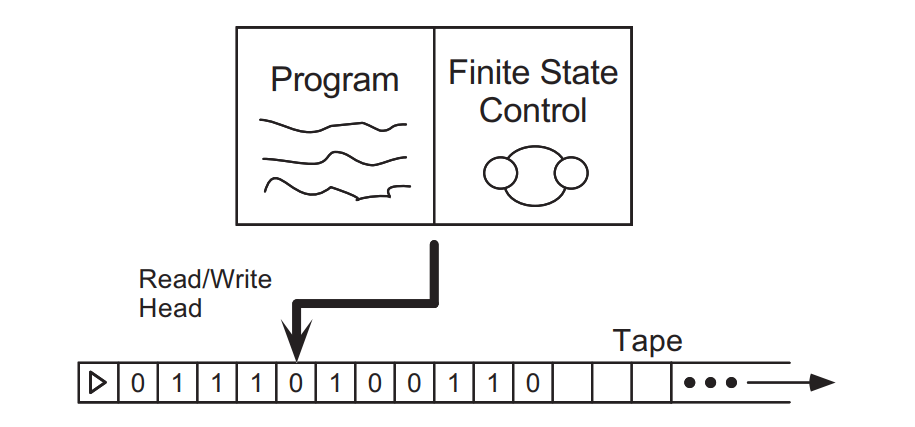
\includegraphics[width=\textwidth]{turing}
\end{figure}
\\ Now we will list an explicit program for computing $f(x)=1$.
Consider the following program:
\begin{enumerate}
    \item $ \left( q_s, s, q_1, s, 1 \right)$
    \item $ \left( q_1, 0, q_1, b, 1 \right)$
    \item $ \left( q_1, 1, q_1, b, 1 \right)$
    \item $ \left( q_1, b, q_2, b, -1 \right)$
    \item $ \left( q_2, b, q_2, b, -1 \right)$
    \item $ \left( q_2, s, q_3, s, 1 \right)$
    \item $ \left( q_3, b, q_h, 1, 0 \right)$
\end{enumerate}

We can see that this program outputs $f(x)=1$ followed by a series of blanks. It is upto you to verify this by tracing the working of the machine line by line.
Although it seems that we certainly did not require such a complex setup to simply compute $f(x) = 1$ the beauty of turing machines lie in the fact that this process can be used to compute various functions ranging from addition, polynomial evaluation to complex arithmetic. Infact all operations that you can do on your current computer can be done on a turing machine. The efficiencies may be different but we are more interested in knowing which problems can indeed be solved on a turing machine.
Church and Turing came up with their thesis, the Church Turing thesis that answers exactly this question.
\begin{thesis}
\textbf{Church Turing Thesis:} The class of functions computable by a Turing machine corresponds exactly to the class of functions which we would naturally regard as being computable by an algorithm.
\end{thesis}
It is to note that this is a hypothesis that has not been proven, however over the last 60 years no counter evidence for the same has been found.
It is interesting to note that quantum computers, and in general, the quantum model of computation do not change the class of functions computable by the model, it merely provides a more efficient way to do so.

Showing that the turing model of computation universally reflects what it means to have an algorithm compute a function is beyond the scope of this report. We will now go through some variations of turing machines. For instance, instead of having just one single tape, the machine could contain two tapes wherein you can use one for the input and other for the output. This variation is identical to the simple turing machine in the sense that both can compute the same set of functions. However for explicitly writing programs for a turing machine it is indeed more convenient to work with the two tape version.
A program line of this turing machine will be of the form $\left(q, x_1, x_2, q^{'}, x_1^{'}, x_2^{'}, d_1, d_2 \right)$ where we will use subscript $1$ for the first tape and $2$ for the other tape.

\begin{exercise}
Write the program lines for a Turing Machine to compute the binary NOT of a binary number provided to you as input in a tape.
(Hint: for such problems it makes more sense to use multiple taped turing machines and more symbols than just $0, 1, b, s$)
\end{exercise}
\begin{exercise}
Describe a Turing program to reverse a binary number provided to you as input in the tape.
\end{exercise}
Another version of a turing machine is a probabilistic turing machine. This machine will transition from one state to another by randomly choosing a state from various possibilities. Note that a deterministic turing machine can in essence simulate a probabilistic machine by going through all possibilities (searching through the search space). Thus they both can compute the exact same class of functions. The probabilistic machine may be more efficient but right now we are only interested in knowing the differences in the set of possible functions computable by different computation models.

Now we describe the circuit model of computation in brief.

\section{Circuit Model of Computation}
The circuit model of computation is essentially the model we are most familiar with, wires and gates that compute binary functions. Taking multiple inputs we can actually compute all kinds of functions which are equivalent to those that can be simulated on a turing machine.  In general our circuits will have gates, which are blocks that compute functions of the form $f : \{0, 1 \}^{k} \to \{0, 1\}^{l}$. However we would like to reduce all our circuits to those made up of some universal blocks. There are a few gates called the universal gates in classical computation that can build up any gate. One such gate is the NAND gate which takes two binary inputs and computes their binary AND and then negates the result.

There are other universal gates as well and some common gates like OR, AND, XOR which are self explanatory. Two other gates are the FANOUT and crossover gates. The FANOUT gate takes an input and copies it out. We will later see that the FANOUT gate has no quantum equivalent because of the \textit{no-cloning} theorem. The crossover gate takes two inputs and simply swaps them.

Later on when we get into quantum circuits, we will show quantum equivalents of these gates and also look at universal quantum gates. It is important to note that quantum mechanics is reversible, infact all of quantum mechanics can be represented as unitary transformations which we will look into in the next section. As a result it is not possible to have irreversible gates in our quantum computational model. So a quantum variant of an AND gate is not possible as AND is irreversible which means that given the output of the AND gate we cannot determine what the inputs were. We reserve this discussion for later when we start dealing with quantum circuits.

\section{Analysis of Computational Problems}

So far we have said that quantum computers provide a more efficient solution of various classical problems. How do we deem which algorithm is better? This section deals with that.

First we talk about orders of magnitude of functions. Let us take an algorithm which scans a list of $n$ numbers and outputs the maximum among them. Clearly such an algorithm takes $n$ operations to finish. In general lesser the number of steps the better the algorithm. But we cannot really talk about the exact number of steps and instead we need an estimate on the number of steps as this value can be variable. Suppose we have an algorithm that scans a list of $n$ numbers to check if $1$ is present or not and if it finds $1$ it terminates. Clearly this can take any number of steps ranging from $1$ to $n$. What we know is that at worst it takes $n$ steps (the upper bound) and in the best case it takes $1$ step (lower bound). So the ideas of upper bound and lower bound on the number of steps provide a rough estimate of how good the algorithm is while average case analysis provide a better picture by accounting for all cases. To talk about such cases in a more formalised manner we use the big-O, big-Omega and big-theta notation.

\begin{definition}
\textbf{Big O} A function $f(n)$ is said to be $O(g(n))$ if there exists some constant c and some $n_0$ such that for all $n \geq n_0$, $$ f(n) \leq cg(n)$$
\end{definition}
An algorithm $A$ is said to have (upper) time complexity $O(g(n))$ if the function $\textbf{TIME}(A(n)) = f(n)$ is $O(g(n))$ where $f(n)$ is the number of steps the algorithm takes on that input.
For example the previous algorithm is $O(n)$ as for $c = 1$ and $n_0 = 1$
$f(n) \leq n$ is satisfied where $n$ is the size of our input.

Similarly we have big theta and big O notations that deal with different bounds.

\begin{definition}
\textbf{Big Theta} A function $f(n)$ is said to be $\Theta (g(n))$ if there exists some constant $c_1, c_2$ and some $n_0$ such that for all $n \geq n_0$, $$c_1g(n) \leq f(n) \leq c_2 g(n)$$
\end{definition}
\begin{definition}
\textbf{Big Omega} A function $f(n)$ is said to be $\Omega (g(n))$ if there exists some constant $c$ and some $n_0$ such that for all $n \geq n_0$ ,$$ c g(n) \leq f(n)$$
\end{definition}

So for instance, the previous algorithm is $\Omega (1)$ and $O(n)$. It is upto you to prove that we cannot have any $\Theta$ bound for this algorithm.
We can also have space complexity where instead of talking about the number of steps, we refer to the number of memory units the program requires. Therefore the previous algorithm has $\Theta (n)$ space complexity as it is using roughly $n$ memory units to store all values (measured as multiples of memory units used to store one number).

Now let us compare the algorithms for prime factorisation. If a number $N$ is given the size of its input is $\log_2 N$. Remember that computer scientists always deal with logarithms to the base 2 as values are stored in binary. So the implicit base is $2$.
Now Shor's algorithm is $O(\log^3 N)$ which is a massive improvement over classical algorithms. A simple trial algorithm is $O(N)$ which becomes exponential in the input size $\log_2 N$. Notice that we are only concerned with the behaviour of the function at large values of the input as computation becomes infeasible only at those limits.

\begin{exercise}
Consider the Merge Sort algorithm. This algorithm can be defined in pseudocode as follows in recursive form (self calling):
\begin{verbatim}
    MERGESORT(List A, SIZE N):
        List B = List A[0, N/2]
        List C = List A[N/2 + 1, N]
        B = MERGESORT(B, N/2) 
        C = MERGESORT(C, N/2)
        A = MERGE(B, C, N/2, N/2)
        return A
\end{verbatim}
The merge function combines the two lists B and C which have half the number of elements that are already sorted and outputs the sorted list formed by combining B and C.

1. Give an $O(N_1 + N_2)$ complexity algorithm for MERGE(List A, List B, Size N_{1}, Size N_{2}).

2. Using the above algorithm write the recursive definition for \textbf{TIME}(List A, Size N) in terms of N. Use this to compute the  time complexity of Merge Sort.
\end{exercise}

\section{Complexity Classes}
\begin{figure}[htp]
    \centering
    \caption{The various complexity classes}
    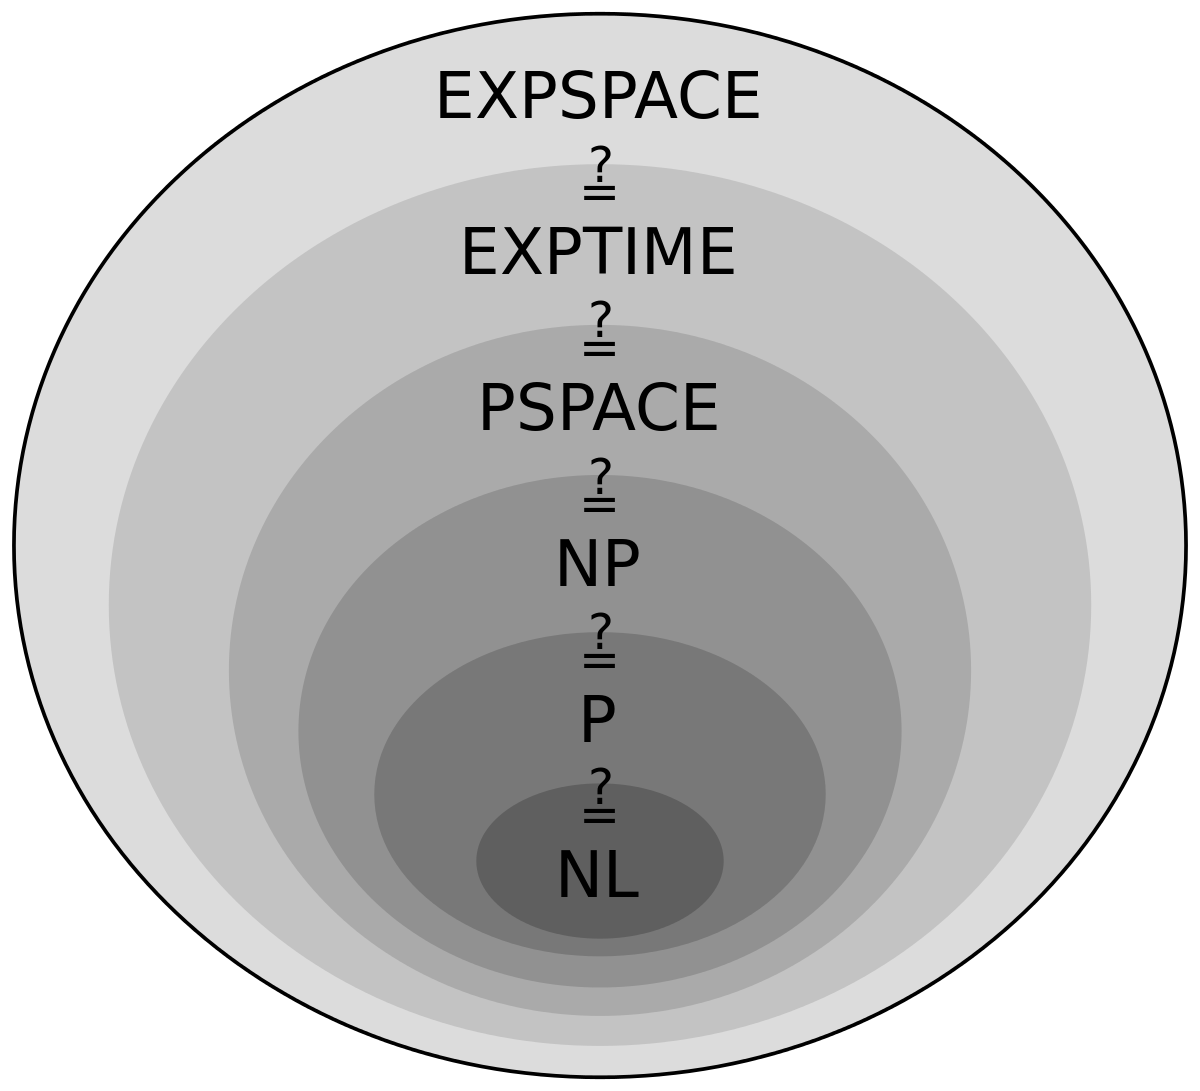
\includegraphics[scale=0.24]{complexity}
\end{figure}
When we covered big-o notation to compare running times of different algorithms we found a way of quantifying the upper bound of the running time. Naturally it makes sense to now categorize different algorithms into different classes on the basis of their running time.

We will start by classifying decision problems, that is problems that have a yes/no answer. These problems provide a lot of insight into the generic case of computable problems and so we stick to them for this report. For instance we may ask the question whether a  number $n$ is a prime or not. This is a decision problem as it has a pure yes/no answer.

To formalize this notion of a decision problem, we rephrase it in terms of a \textit{language} L. A language is a subset of all possible strings formed from a subset of characters which we term as alphabets. For instance we may define the \textit{prime} language $L_P$ as the subset of all possible strings formed from $\{0, 1\}$ such that the corresponding binary number is a prime.

Then we can rephrase decision problems into creating a Turing Machine (or an algorithm) that will output yes if the corresponding input is part of that language and else no. These outputs can be two end states of the turing machine $q_y, q_n$.

A complexity class is a set of problems that satisfy a particular property with respect to its time or space or energy complexity.
For an algorithm (or a machine implementing it) $A$ solving a decision problem $D$ we say that $D \in \textbf{P}$ where \textbf{P} is a complexity class if for an input of size $n$, \textbf{TIME}(A(n)) $ = O(n^k)$ for some $k>0$.
Roughly $\textbf{P}$ is the collection of those decision problems where the decision can be found out in polynomial size of the input.

\textbf{P} is an important complexity class as it contains those problems that we can solve in a reasonable amount of time compared to say exponential or factorial growth algorithms. 

Another important complexity class is \textbf{NP}. Roughly speaking it is that collection of decision problems whose truth value can be verified with the help of another input called the witness W in polynomial size of the main input.
Formally a decision problem is in \textbf{NP} if
\begin{enumerate}
    \item given x $\in $ L, there exists a witness W such that using the W a turing machine can deterministically state that x $\in$ L by going to the positive state $q_y$ in time proportional to a polynomial in size of x.
     \item given x $\not\in $ L, for all possible witnesses W the turing machine will deterministically state that x $\not\in$ L by going to the  state $q_n$ in time proportional to a polynomial in size of x.
\end{enumerate}

For example consider the decision problem $D$ asking whether a number $x$ is \textbf{NOT} in the prime language, that is $ x \in L_P^{'}$ that we previously described. Then a possible witness could be a factor of the number $x$ where we check if the witness divides the number (where the witness is not $x$ or 1). If $x$ was a prime then for any possible witness we cannot use it to say that witness divides the number  and so the second condition is met. Thus this problem is in \textbf{NP}.

In general it is not easy to provide a witness for the complement of a language. For example in the previous case the complement would be the language of primes. There, coming up with a witness that gives a guarantee that $x \in L_P$ is not easy.

\begin{exercise}
Prove that \textbf{P} $\subseteq$ \textbf{NP}
(Hint: it is not necessary to use the witness always)
\end{exercise}
It is not yet known whether  \textbf{P} $\neq$ \textbf{NP} and this is infact a millennium problem. 
There are other complexity classes related in terms of space. \textbf{PSPACE} refers to those problems which take polynomial space while \textbf{EXPSPACE} take exponential space. Similarly we have \textbf{L} for logarithmic time complexity and \textbf{LSPACE} for logarithmic space complexity.

\begin{exercise}
Prove that $\textbf{P} \subseteq \textbf{PSPACE}$
\end{exercise}
With respect to probabilistic turing machines, we have \textbf{BPP} which contains all those decision problems which we can be probabilistically solved in polynomial time with probability atleast $k$ where $k > \frac{1}{2}$. However this $k$ can be made as close to $1$ as we desire by running the algorithm many times for the same input and choosing the maximum occurring result. Thus \textbf{BPP} is more indicative of "fast" solvable problems than \textbf{P} in practice.
We end this section by allauding to another complexity class of particular interest to this, \textbf{BQP}. \textbf{BQP} is the quantum equivalent of \textbf{BPP}, that is those decision problems that can be solved with a high degree of probability $ > \frac{1}{2}$ using a quantum circuit taking time which is polynomial in the size of the input.

\clearpage